\section{Approach}

\subsection{Algorithm}

\begin{frame}{Important Variables} % ___________________________________________

Description of the main variables

  \begin{table}[h]
    \begin{center}
      \begin{tabular}{c|l}
      \cellcolor{white} Variable Name & Description \\ % adding \cellcolor{} here fixes the vertical line between the columns for some reason
      \rowcolor{LightGray}
      $D$ & Depth image from RGB-D sensor \\
      $P$ & Pose of the sensor \\
      \rowcolor{LightGray}
      $D_n$ & Parts of $D$ that are \emph{novel} \\
      $S$ & Novel surface generated from $D_n$ \\
      \rowcolor{LightGray}
      $M$ & Global mesh \\
      \end{tabular}
    \end{center}
  \end{table}

\end{frame}

\note[itemize]{
\item $D$ - an image
\item $P$ - Describes position and orientation of sensor
\item $D_n$ - Subset of point in $D$ that have been labeled as novel
\item $S$ - Mesh structure. List of vertices and elements.
\item Vertices are points and elements define connections between vertices
}

\begin{frame}{MABDI Algorithm} % _______________________________________________
  \vspace{-0.13in}
  \includegraphics[height=0.95\textheight]<1>
    {../figures/presentation/approach_mabdi_algorithm_p0.pdf}
  \includegraphics[height=0.95\textheight]<2>
    {../figures/presentation/approach_mabdi_algorithm_p1.pdf}
  \includegraphics[height=0.95\textheight]<3>
    {../figures/presentation/approach_mabdi_algorithm_p2.pdf}
  \includegraphics[height=0.95\textheight]<4>
    {../figures/presentation/approach_mabdi_algorithm_p3.pdf}
  \includegraphics[height=0.95\textheight]<5>
    {../figures/presentation/approach_mabdi_algorithm_p4.pdf}

    \note<2>{\begin{itemize}
      \item[] The MABDI algorithm
      \item Orange -
      \item Input to the algorithm. This has been simulated for this work.
      \item Classification -
      \item What sets MABDI apart from traditional mesh-based mapping algorithms.
      \item Allows us to classify data before it is added to the Global Mesh.
    \end{itemize}}

  \note<2>{\begin{itemize}
    \item[] Input
    \item Has been simulated in this work.
    \item We will cover simulation process in detail.
    \item[] Generate Expected Depth Image
    \item Takes the global mesh (what we know about the environment)
    \item And pose of sensor.
    \item Generates what we expect to see.
    \item Meaning what would a RGB-D sensor would see.
    \item Given what we know about the environment and the pose of the sensor.
  \end{itemize}}

  \note<3>{\begin{itemize}
    \item[] Classify Depth Image
    \item This is the heart of MABDI
    \item and is MABDI's contribution to the state-of-the-art
    \item Determine which points from D are novel.
    \item (From a new part of the environment that has not been seen before)
    \item Taking the absolute difference between $E$ and $D$ and thresholding.
    \item (point to equation)
    \item If the differences are small, those points are thrown away.
    \item If the differences are large, those points are kept.
    \item If the difference is large, the measurements are coming from a part of the environment that has not been seen before.
  \end{itemize}}

  \note<4>{\begin{itemize}
    \item[] Surface Reconstruction
    \item Create a mesh structure from the novel points
    \item Cover in detail next
  \end{itemize}}

  \note<5>{\begin{itemize}
    \item Add Novel Surface to Global Mesh
    \item Append surface to the global mesh
    \item that is continuously being updated
  \end{itemize}}

\end{frame}

\begin{frame}[plain]
  \begin{center}
    {\huge Implementation Specific Details}
  \end{center}
\end{frame}


\subsection{Surface Reconstruction}

\begin{frame}{Initial Mesh} % __________________________________________________
  \only<1>{\begin{itemize}
    \item Surface Reconstruction component is responsible for creating $S$ from $D_n$
    \item Our Method:
    \item Define topology in 2D, on the depth image
    \item Project to 3D
    \item Remove elements
  \end{itemize}}

  \begin{center}
    \includegraphics[height=0.90\textheight]<2>
      {../figures/approach_sr_topology.pdf}
  \end{center}

  \includegraphics[width=\textwidth]<3>
    {../figures/presentation/approach_project_p.pdf}

  \note<1>{\begin{itemize}
    \item Responsible for creating a surface $S$ from the novel points $D_n$
    \item $S$ is a mesh data structure that consists of a list of vertices and elements
    \item - Vertices are points
    \item - Elements define connections between vertices
    \item []
    \item Generate initial mesh with all points in $D$
    \item Depth image
    \item - Not a set of unorganized points
    \item - Has structural information
    \item - This allows us to define a topology in 2D that is preserved when projected to 3D
  \end{itemize}}

  \note<2>{\begin{itemize}
    \item Imagine this is the depth image
    \item - Every blue point is a pixel in the depth image
    \item - Corresponds to 3D point in space
    \item Depth image
    \item - Not a set of unorganized points
    \item - Has structural information
    \item - This allows us to define a topology in 2D that is preserved when projected to 3D
    \item We then take every blue dot and project them into 3D space
    \item preserving the connections between vertices
  \end{itemize}}

  \note<3>{\begin{itemize}
    \item Imagine mesh being defines using every pixel in depth image
    \item Then projected to 3D space
    \item - Ignore the background for now
    \item Note there will be no surface
    \item behind the cup,
    \item under the table,
    \item anywhere on the floor that the sensor doesn't see
  \end{itemize}}
\end{frame}


\begin{frame}{Removing elements} % _____________________________________________
  \only<1>{
    Elements are removed from the $S$ if they touch pixels from the sets:
    \begin{itemize}
      \item $D_{known}$
      \item $D_{boundary}$
      \item $D_{invalid}$
    \end{itemize}
  }

  \begin{center}\only<2->{
  \includegraphics[height=0.90\textheight]<2>
    {../figures/presentation/approach_sr_pts_0.pdf}
  \includegraphics[height=0.90\textheight]<3>
    {../figures/presentation/approach_sr_pts_1.pdf}
  \includegraphics[height=0.90\textheight]<4>
    {../figures/presentation/approach_sr_pts_2.pdf}
  \includegraphics[height=0.90\textheight]<5>
    {../figures/presentation/approach_depth_image_p.pdf}
  }\end{center}

  \note<2>{\begin{itemize}
    \item Inside the circle represents the set
    \item containing every point from $D$
  \end{itemize}}

  \note<3>{\begin{itemize}
    \item $D_n$ (novel) is everything that the categorization process said is novel.
    \item (point to equation)
  \end{itemize}}

  \note<4>{\begin{itemize}
    \item We define two additional set of points to be thrown away.
    \item $D_{boundary}$
    \item - remove elements defined by points that lie on completely different surfaces
    \item $D_{invalid}$
    \item - elements that are out of range of the sensor
  \end{itemize}}

  \note<5>{\begin{itemize}
    \item We define two additional set of points to be thrown away.
    \item $D_{boundary}$
    \item - (point out neighboring pixels on leg and floor)
    \item $D_{invalid}$
    \item - (point out background)
  \end{itemize}}
\end{frame}

\begin{frame}{Removing elements - $D_{known}$} % _______________________________
  \begin{gather*}
    D_n = \lvert D - E \rvert > threshold \\ \\
    D_{known} = D \setminus D_n
  \end{gather*}
  \note{\begin{itemize}
    \item Define novel and known points formally
    \item $D_n$ - Same equation as discussed "Classify Depth Image" component
    \item $D_{known}$
    \item - All the points that not novel
    \item - Those points that have a small difference
  \end{itemize}}
\end{frame}

\begin{frame}{Removing elements - $D_{boundary}$} % ____________________________
  \begin{gather*}
    K = \begin{bmatrix} 2 & -1 \\ -1 & 0 \end{bmatrix} \\ \\
    D_{boundary} = (D \ast K) > threshold
  \end{gather*}
  \note{\begin{itemize}
    \item Lie on different surfaces
    \item Like the pixel neighbors floor and leg that we discussed
    \item[]
    \item Two dimensional, differencing convolution filter is passed over $D$
    \item This filter has a magnified response at points where the difference
    between neighboring pixels is large
    \item Remembering pixel values signify depth
  \end{itemize}}
\end{frame}

\begin{frame}{Removing elements} % _____________________________________________
  \begin{center}
    \includegraphics[height=0.90\textheight]<1>
      {../figures/presentation/approach_sr_pts_2.pdf}
    \includegraphics[height=0.90\textheight]<2>
      {../figures/approach_sr_element_removal.pdf}
  \end{center}
  \note<1>{\begin{itemize}
    \item Each colored circle represents points that we are going to remove
  \end{itemize}}
  \note<2>{\begin{itemize}
    \item Points from the colored circle are represented as the red points
    \item Technically, these points have already been projected to 3D
    \item but this is the best way to visualize this concept
  \end{itemize}}
\end{frame}

\subsection{Software Design}

\begin{frame}{Diagram} % _______________________________________________________
  \begin{center}
  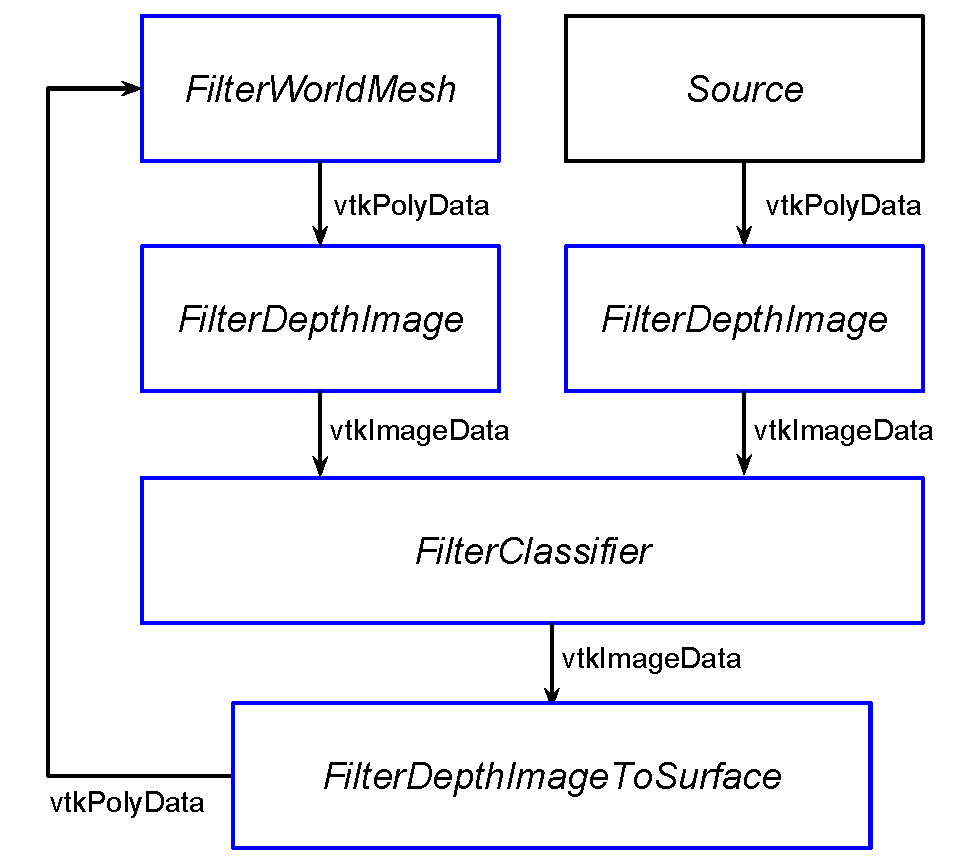
\includegraphics[height=0.90\textheight]
    {../figures/approach_software_diagram.pdf}
  \end{center}
  \note<1>{\begin{itemize}
    \item In blue are the core components
    \item In black components for the simulation of a real environment
  \end{itemize}}
  \note<2>{\begin{itemize}
    \item  \textit{Source}
    \item - Define the environment that is used for the
    \item \textit{FilterDepthImage}
    \item - Render the incoming vtkPolyData in a window and
    \item - output the depth buffer from the window as a vtkImageData
    \item - output has pose information of the sensor.
  \end{itemize}}
  \note<3>{\begin{itemize}
    \item \textit{FilterClassifier}
    \item - Implements the true innovation of MABDI
    \item - take difference of actual and expected
    \item - outputs a new depth image where the data that is not novel is marked
    to be thrown away
    \item \textit{FilterDepthImageToSurface}
    \item - Performs surface reconstruction
    \item - surface is output as a vtkPolyData.
    \item \textit{FilterWorldMesh}
    \item - Here we simply append the incoming novel surface to a growing global
    mesh that is also output as a vtkPolyData
  \end{itemize}}
\end{frame}
